\documentclass[prl,aps,twocolumn,floatfix,amsmath,amssymb,superscriptaddress,tightenlines]{revtex4}
\usepackage{graphicx}
\usepackage{epstopdf}
\usepackage{amsfonts}
\usepackage{bm}
\usepackage{color}
\usepackage{ulem}
\begin{document}

\date{\today}
\title{Emergent chord length in the entanglement entropy of
  two-dimensional gapless systems}

\author{Hyejin Ju}
\affiliation{University of California, Santa Barbara, CA, 93106}

\author{Ann B. Kallin}
\affiliation{Department of Physics and Astronomy, University of Waterloo, Ontario, N2L 3G1, Canada} 

\author{Paul Fendley}
\affiliation{Physics Department, University of Virginia,
  Charlottesville, VA 22904}
\affiliation{Microsoft Research, Station Q, CNSI Building, University of California, Santa Barbara, CA, 93106}

\author{Matthew B. Hastings}
\affiliation{Microsoft Research, Station Q, CNSI Building, University of California, Santa Barbara, CA, 93106}

\author{Roger G. Melko}
\affiliation{Department of Physics and Astronomy, University of Waterloo, Ontario, N2L 3G1, Canada} 

\begin{abstract} 
We show that the entanglement entropy of a variety of two-dimensional
gapless systems contains a logarithmic term that depends on the size
of the ``bulk''. Precisely, we show that the Renyi entropy between two
regions of length $l$ and $L-l$ extending around a cylinder of length
$L$ depends on $\ln(\sin(\pi l/L))$. This logarithmic term is thus
akin to that appearing in 1d systems with conformal symmetry. We
illustrate this with numerical results on the Heisenberg model with
N\'eel order, a free Dirac fermion, and the nearest-neighbor RVB wave
function.


 
\end{abstract}
\maketitle

{\it Introduction.} It is now well established that the low-energy physics of certain one-dimensional (1D) quantum many-body systems can be described by relativistic 1+1 dimensional field theories.  This correspondence occurs at quantum critical points, where in addition to scale invariance, quantum systems typically enjoy {\it conformal} invariance.  In 1D, this has allowed classification of quantum critical points via the appropriate 1+1 dimensional conformal field theory (CFT): in particular the central charge $c$ describing the CFT.
In the cases where it is not known exactly (in integrable models), 
this central charge can be obtained directly in numerical measurements of the Renyi entanglement entropy,
$
S_n = 1/(1-n) \ln \big[ {\rm Tr} \rho_A^n \big],
$
(where region $A$ is entangled with its complement, region $B$), has become commonplace in simulations using the density matrix renormalization group (DMRG).  In particular, the
scaling of the Renyi entropy at a 1D critical system, with total length $L$ and length of region $A$ being $x$, obeys
\begin{equation}
S_n = \frac{c}{6}\left({ \frac{1}{1+n} }\right) \ln\Big[ \frac{L}{\pi} \sin\big( \frac{\pi x}{L} \big) \Big]. \label{1Dcft}
\end{equation}
Numerical measurement of $c$ via Eq.~\ref{1Dcft} has become the gold standard, since it is accessible in one simple measurement which gives access to the most important universal signature of the underlying CFT.

In higher dimensions, the relationship between entanglement entropy and universal quantities is less concrete.  Although conformal symmetries exist at scale-invariant critical points in the presence of translational and rotational symmetry, the breaking of the latter in physical systems can make them non-conformal.  Arguments exits that logarithms similar to Eq.~(\ref{1Dcft}) should emerge due to some asymptotic restoration of conformal invariance in higher-dimensional gapless models, although counter examples are known.  This nonetheless often leads to the hope that a logarithmic scaling of entanglement entropy can be used to define an ``effective'' central charge for non-conformally invariant systems that may contain universal physics (or the equivalent of Zamolodchikov's $c$-theorem in higher-dimensions).

{\it \color{red} Ann's section below}:
{\color{red} RELATE HEISENBERG AND RVB - type below here}

Using quantum Monte Carlo (QMC) techniques we simulate both the Heisenberg ground state and the resonating valence bond (RVB) wavefunction in two dimensions (2D). 
% heisenberg projector algorithm
The Heisenberg ground state is projected from a trial state by applying a high power of the Hamiltonian, via QMC in the valence bond (VB) basis.\cite{Sandvik_VBQMC}
The VB operators act to reorganize the bonds while effectively penalizing states with longer bonds.
% rvb algorithm
The RVB wavefunction contains all possible combinations of only nearest-neighbor VBs in an equal superpositions.
The RVB QMC algorithm does a random walk through the possible states by creating a defect at some point and propagating it through the system (thereby rearranging the nearest-neighbor bonds) until the defect reaches the initial point and its path forms a closed loop.
% wavefunctions are related
If we visualize the Heisenberg ground state in this VB language, then the RVB wavefunction is its largest component, the remainder of the state being equal superpositions with longer bonds decaying as $1/r^3$ \cite{Sandvik_VB_decay} with the length of the bonds.

%geometry
Within both these systems (Heisenberg and RVB) we use a square lattice torus geometry and measure the entanglement for two different types of region $A$.

{\color{red} END - and above here}

 \begin{figure}[h]
   \begin{center}
   \scalebox{1}{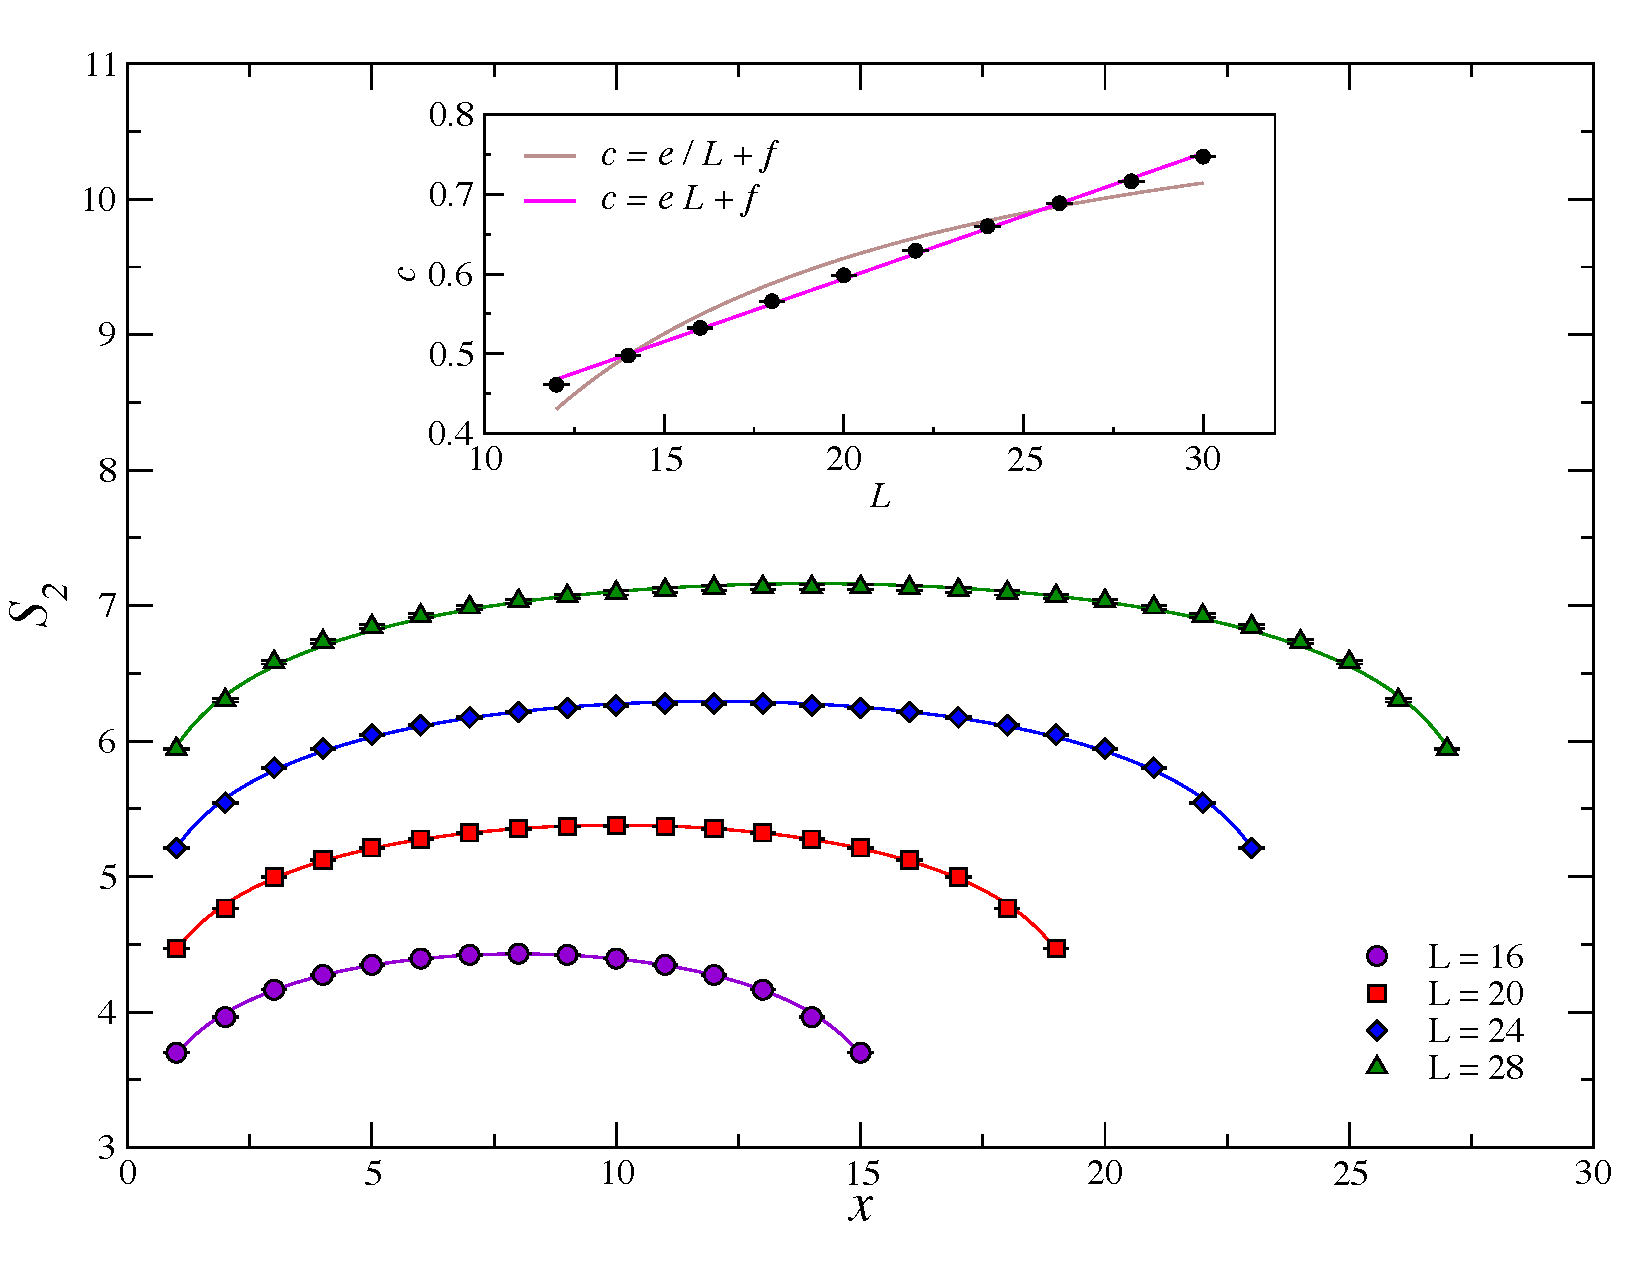
\includegraphics[width=\columnwidth]{./figs/heisenberg.pdf}}
   \end{center}
   \caption{Heisenberg Renyi-bow. }
   \label{fig:1}
 \end{figure}

 \begin{figure}[h]
   \begin{center}
   \scalebox{1}{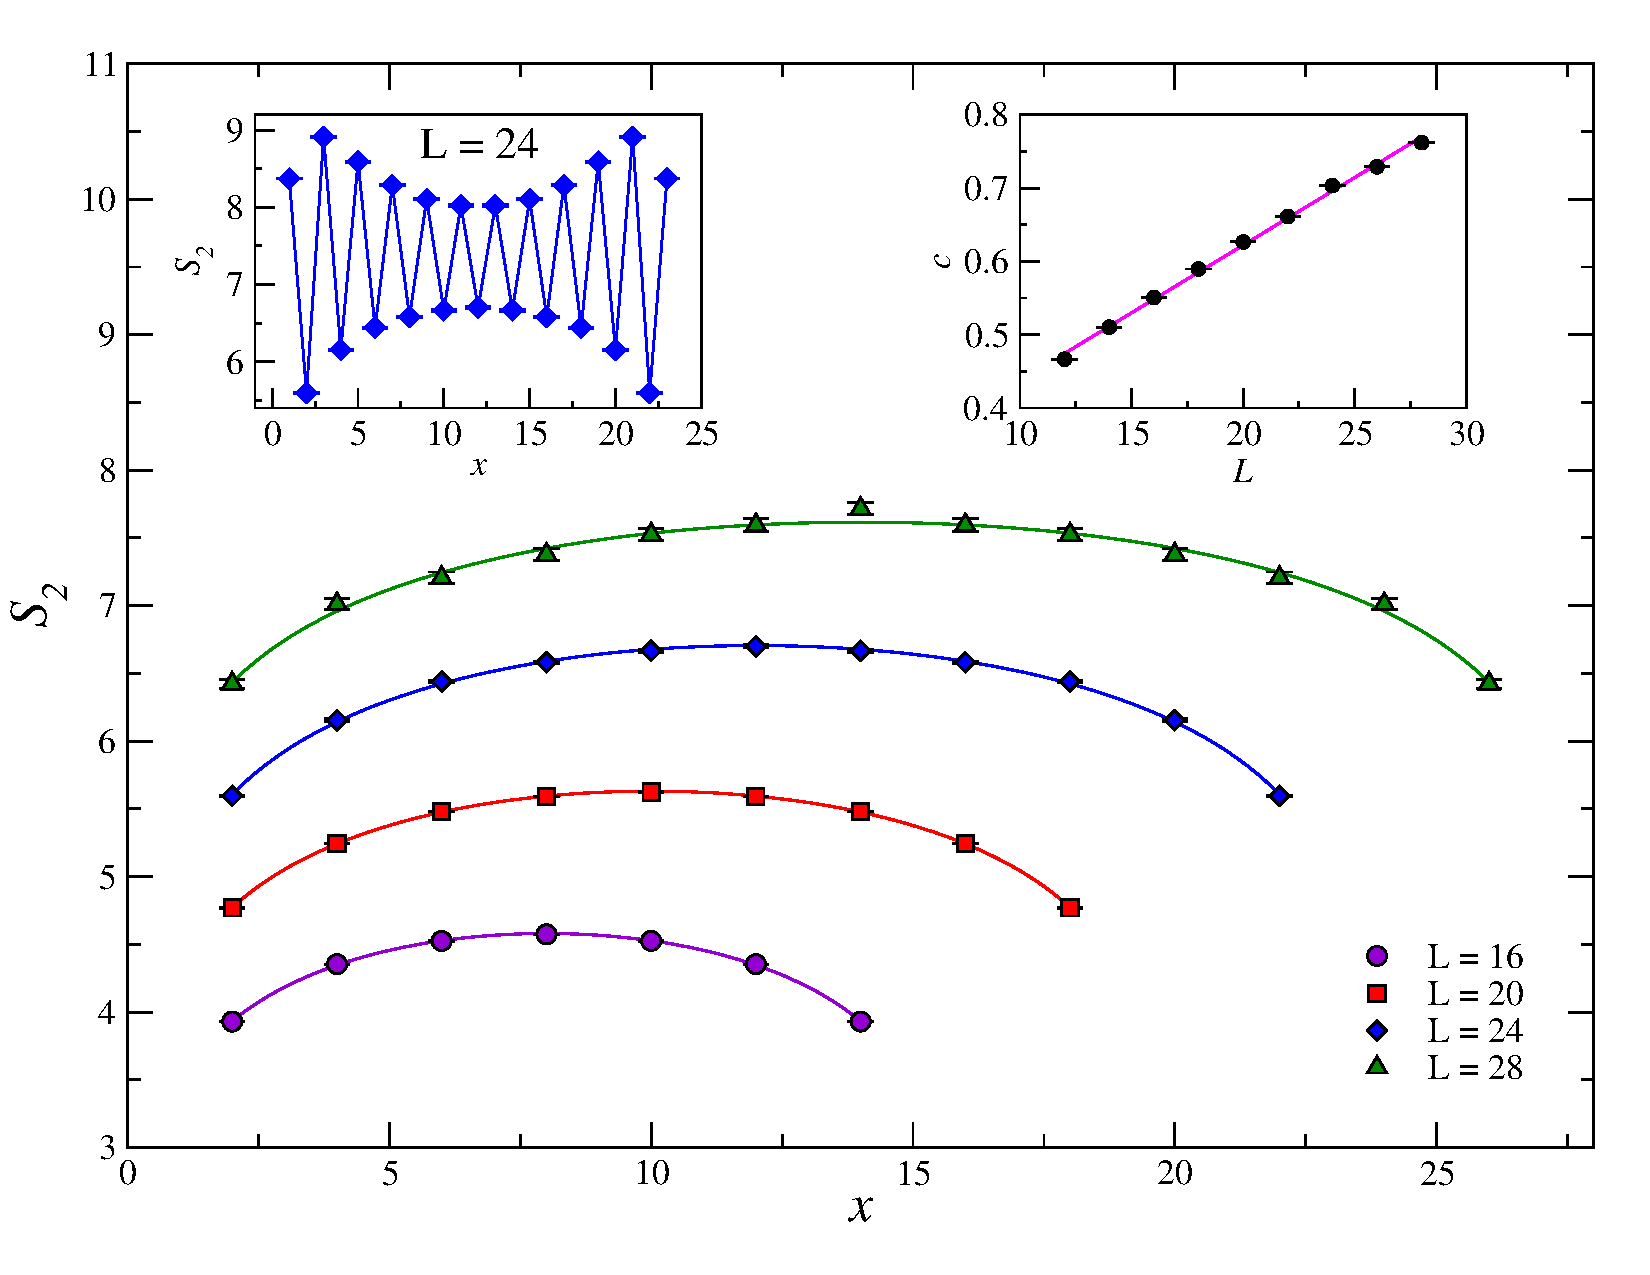
\includegraphics[width=\columnwidth]{./figs/rvb.pdf}}
   \end{center}
   \caption{RVB Renyi-bow. }
   \label{fig:1}
 \end{figure}



\bibliography{Biblio}

\end{document}
